\documentclass{article}
\usepackage[margin = 1in, footskip = 0.25in]{geometry}
\usepackage{amsfonts}
\usepackage{amsmath}
\usepackage{amsthm}
\usepackage{amssymb}
\usepackage[ruled,vlined]{algorithm2e}
\usepackage{xcolor}
\usepackage{listings}
\usepackage{graphicx}

\usepackage{xparse}

\NewDocumentCommand{\codeword}{v}{%
\texttt{\textcolor{teal}{#1}}%
}
\lstset{language=C,keywordstyle={\bfseries \color{blue}}}

\renewcommand{\familydefault}{\sfdefault}
\newcommand{\bc}{\text{\sc bc}}
\newcommand{\HH}{\smash{\widetilde{H}}}

\title{Code details}
\date{}

\begin{document}
\maketitle
This document provides an overview of main functions and their outputs. Those interested in contributing to the project may find this document useful.

\section{The persistent extension method}
\subsection{Implementation}
\begin{itemize}
\item The persistent extension method is implemented in 6 different functions:	
	\begin{itemize}
	\item \codeword{run_extension_VR_to_VR()}
	\item \codeword{run_extension_VR_to_VR_bar()}
	\item \codeword{run_extension_VR_to_W()}
	\item \codeword{run_extension_VR_to_W_bar()}
	\item \codeword{run_extension_W_to_VR()}
	\item \codeword{run_extension_W_to_VR_bar()}
	\end{itemize}
\item The functions implement a variation of the cycle-to-bars extension (Algorithm 5 from paper) or a bar-to-bars extension (Algorithm 3 from paper). The ones implementing bar-to-bars extension has the string \codeword{_bar} at the end of its function name.
\item All implementations are component-wise extensions with $\mathbb{F}_2$ coefficients.
\item Due to computation speed issues, the functions do not return the full collection of cycle extensions and bar extensions as described in the paper. Instead, the functions return the baseline and offset cycle extensions and bar extensions. The output of the above functions can then be processed to return the full collection of cycle extensions $E(\tau, Y^{\bullet})$ and bar extensions $S(\tau, Y^{\bullet})$.  
\item The algorithm below summarizes the bar-to-bars extension method variation implemented by our functions. The cycle-to-bars extension functions implement a similar variation. 
\end{itemize}
%------------------------------------------------------------------------------------------------------------------------------
\begin{algorithm}[H]
\caption{Bar-to-bars extension method variation}
\label{alg_variation}
\textbf{Input}:
\begin{itemize}
    \item filtered simplicial complexes $Z^{\bullet}$, $Y^{\bullet}$ on vertex set $P$, 
    \item a bar $\tau \in \bc_k(Z^{\bullet})$
    \end{itemize}

\textbf{Steps:}
\begin{enumerate}
\item Fix interval decompositions $\mathcal{B}$ of $P\HH_k(Z^{\bullet})$ and $\mathcal{D}$ of $P\HH_k(Y^{\bullet}).$
\item Find parameter $\delta(\tau)-1$ and cycle $[\tau_*^{\mathcal{B}}]$.
\item Let $p_Y$ be the collection of parameters from Algorithm 1 of paper run with inputs $\delta(\tau)-1$ and $[\tau_*^{\mathcal{B}}]$. 
\item Let $\text{\sc{bars}}_{\tau}^{\mathcal{F}} = \{ \rho_1, \dots, \rho_m \}$ be the set of bars in the $\mathcal{F}$-bar representation.
\item For each $\ell \in p_Y$:
	\begin{enumerate}
	\item Find the baseline cycle extension $\mathfrak{E}_{\ell}^{\text{baseline}} = \Upsilon_{\ell}(\sum_{i=1}^m [\rho_i^{\mathcal{F}, \ell}])$
	\item Find the offset cycle extension $\mathfrak{E}_{\ell}^{\text{offset}} = \{ \Upsilon_{\ell}[\rho^{\mathcal{F}, \ell}] \; | \; \rho \in \text{\sc{bars}}_{\text{short}}^{\ell}\} $
	\item Find the baseline bar extension  $B^{\ell} = \{ S^{\mathcal{D}}_{[t]} \; | \; [t] \in \mathfrak{E}_{\ell}^{\text{baseline}} \}$ .
	\item Find the offset bar extension $O^{\ell} = \{ S^{\mathcal{D}}_{[t]} \; | \; [t] \in \mathfrak{E}_{\ell}^{\text{offset}} \}$.
	\end{enumerate}

\item Return $\mathfrak{E}_{\ell}^{\text{baseline}}, \mathfrak{E}_{\ell}^{\text{offset}}, B^{\ell}$, and $O^{\ell}$ for $\ell \in p_Y$.
\end{enumerate}
\end{algorithm}


\begin{itemize}
\item The following flow chart summarizes the key functions implemented in each step. The left-most column describes the general flow. The remaining columns show the explicit functions called to execute the specific task. Depending on the filtration types, the component functions require slight modifications.
\end{itemize}

\begin{figure}[h!]
\centering
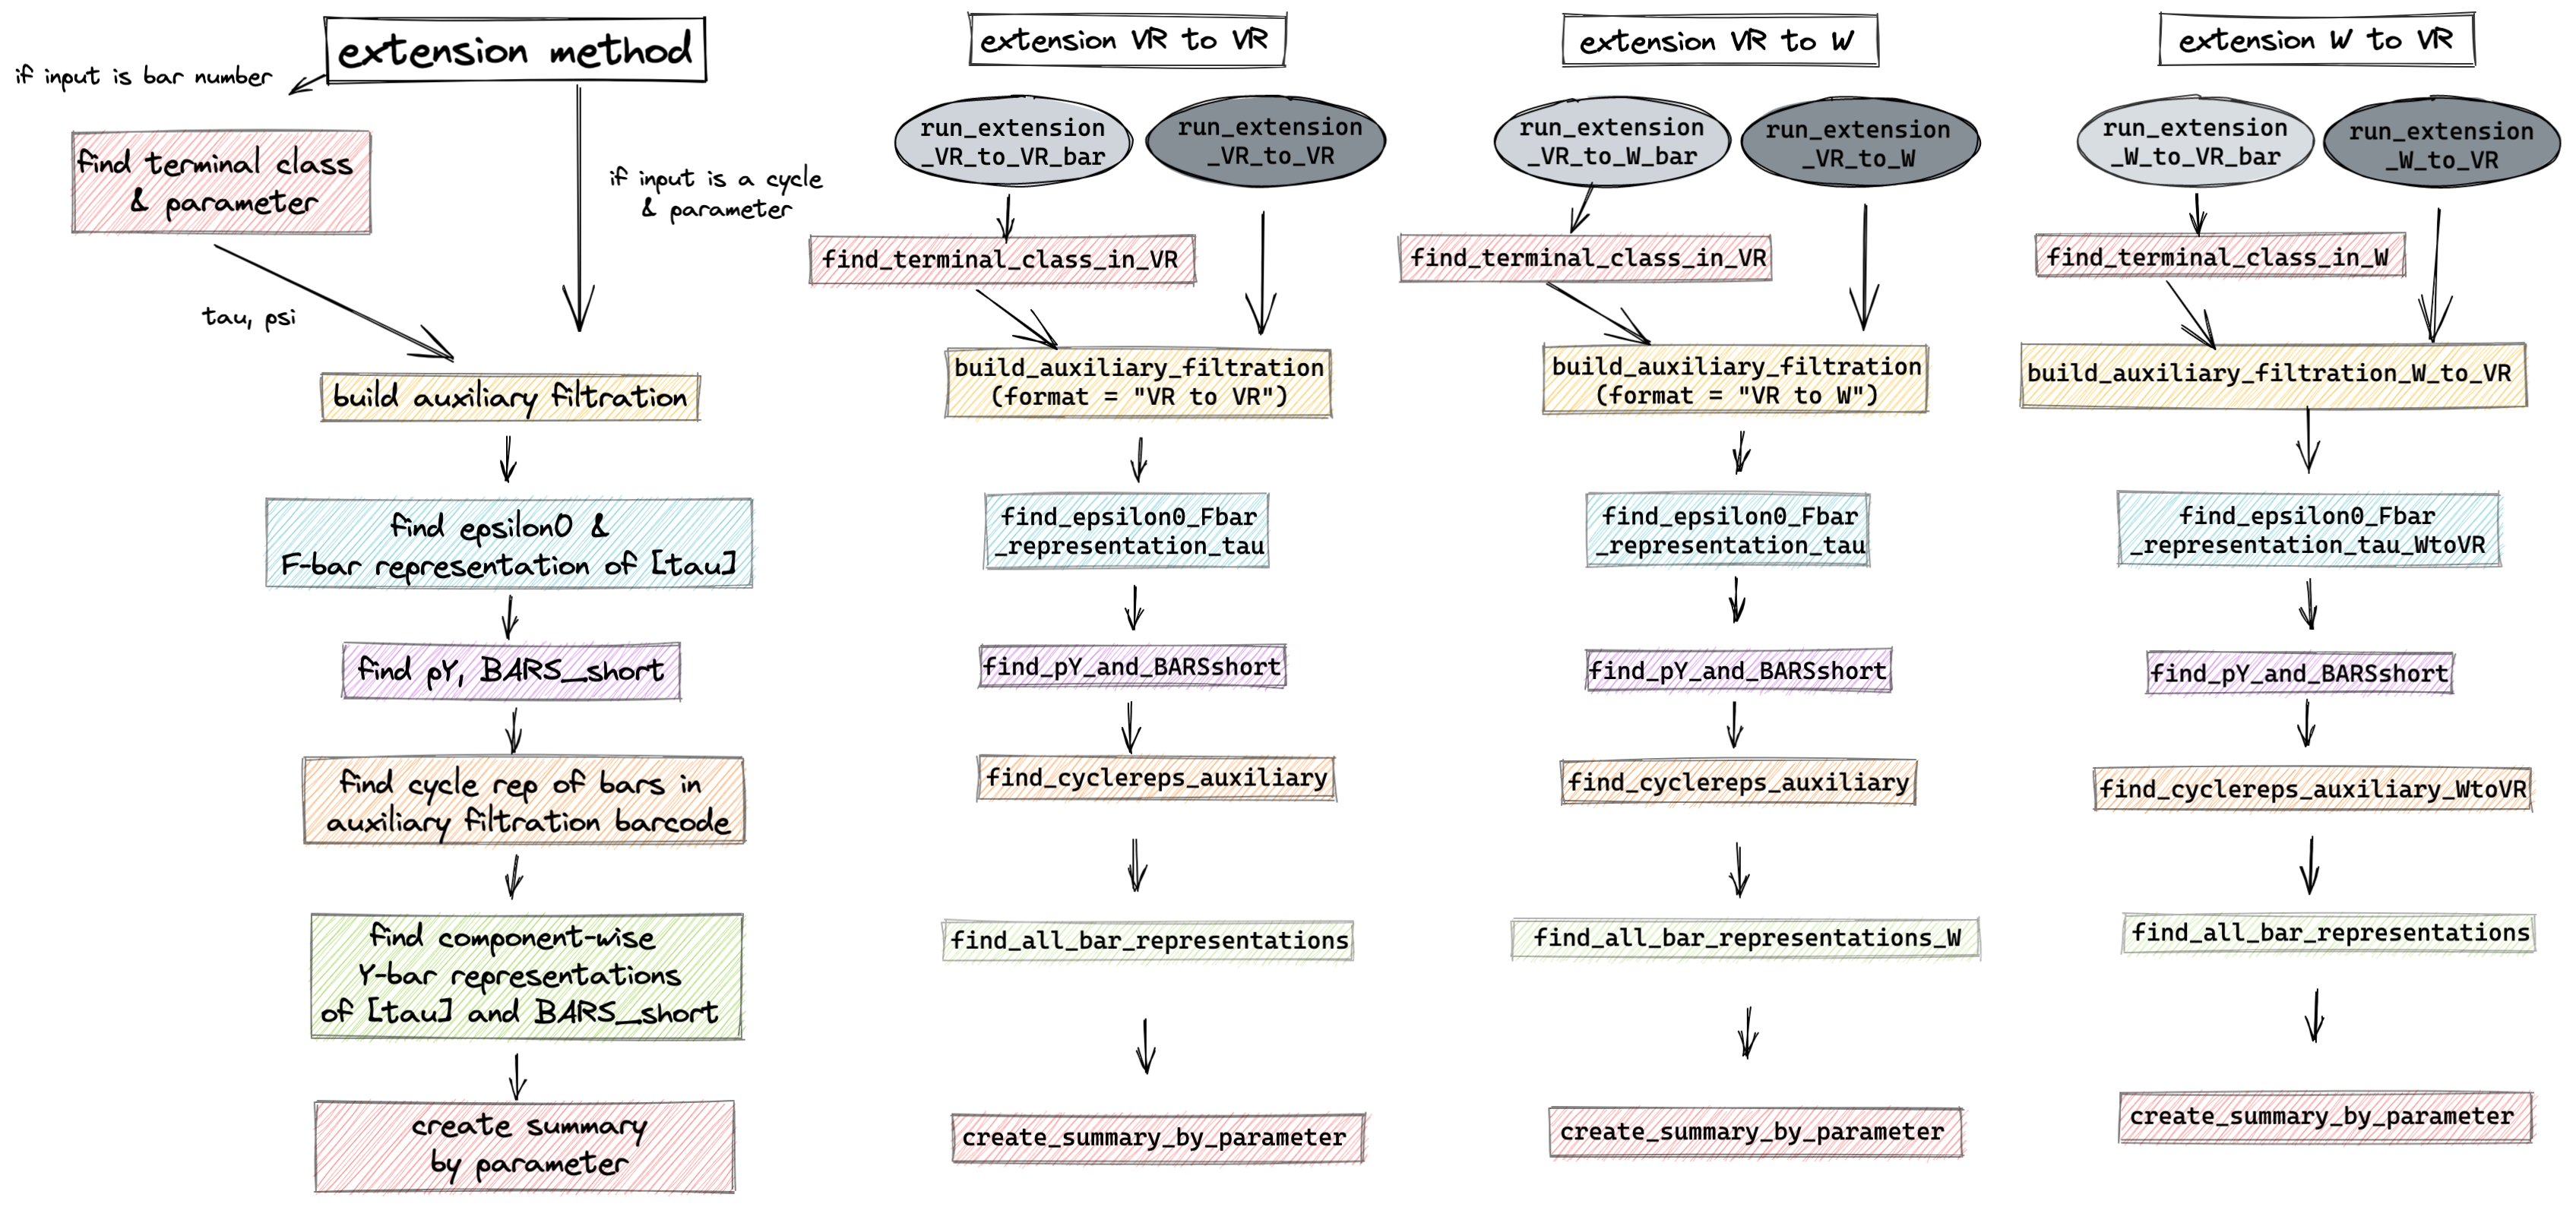
\includegraphics[width = \textwidth]{code_components.png}
\end{figure}

\begin{itemize}
\item If you choose to take a closer look at the code, you will notice that there are many functions and variables that keeps track of the various ways in which we describe a simplex (and therefore, a chain). Here are some things to keep in mind:
\begin{itemize}
\item A simplex can either be expressed using some index (the ``i"-th simplex) or it can be expressed using its 0-simplices ($ s = [v_0, v_1]$). We'll refer to the former as the ``index notation" and the latter as the ``simplex notation". Any functions and variables with the t erm \codeword{simplex2index} or \codeword{index2simplex} will convert one notation to another.
\item The vertex ordering used in various functions may differ from the vertex ordering provided by the input. That is, let's say we provide a distance matrix $D$. We would intuitively think that the 1st row of $D$ corresponds to vertex $v_1$, 2nd row of $D$ corresponds to vertex $v_2$, and so on. However, the vertex ordering used in the computations may differ from the order of the rows of $D$. This is because Eirene permutes the vertices during its computations. We often use specific permutations to go back and forth between Eirene's vertex ordering and the default vertex ordering. 
\item When building the Witness complex from a cross-distance matrix $D_{P,Q}$, it's possible to provide the maximum parameter at which to build the Witness complex. In such cases, one may end up using only a sub-collection of the vertices provided by the rows of $D_{P,Q}$. In such cases we end up with two distinct ordering of the vertices: The ordering provided by the distance matrix $D_{P,Q}$ and the ordering among the sub-collection of vertices used to build the Witness complex. The former is called the \codeword{default_vertex} and the latter is called the \codeword{Wepsilon_vertex} in the code.
\end{itemize}

\end{itemize}

%========================================================================
\subsection{Finding the full collection of cycle extensions and bar extensions}
\begin{itemize}
\item As noted in the previous section, the 6 extension method function returns the \textbf{component-wise} cycle and bar extensions. We provide several functions that help the user to find the full collection of cycle extensions ($E(\tau, Y^{\bullet})$ from paper) and bar extensions ( $S(\tau, Y^{\bullet})$ from paper) .
\item We first discuss methods for finding the collection of cycle extensions $E(\tau, Y^{\bullet})$ and the bar extensions under a \textbf{fixed interval decomposition} of $P\HH_k(Y^{\bullet})$. We'll then discuss methods for finding the full bar extensions under any interval decomposition of $P\HH_k(Y^{\bullet})$. 
\item In each section, we present multiple functions that achieve the same goal. The appropriate use of the functions depend on the size of the data -- In particular, the number of bars in $\bc_k(Z^{\psi} \cap Y^{\bullet})$ and $\bc_k(Y^{\bullet})$. 
\end{itemize}

\subsubsection{Finding all cycle extensions and bar extensions under fixed target interval decomposition}
\begin{itemize}
\item Use the function \codeword{return_extension_results_at_parameter()} for an interactive exploration of baseline and offset bar extensions. For each parameter, user can select which offset bar extensions to include in their final view. 
\item To find all cycle extensions and bar extensions at a specific parameter, run the function \codeword{find_CE_BE_at_param()}. 
\item To find all cycle extensions and bar extensions at all parameters, run \codeword{find_CE_BE()}.
	\begin{itemize}
	\item Let \codeword{CE}, \codeword{BE} be the outputs of the function.
	\item Given a parameter \codeword{param}, and some index \codeword{i}, \codeword{CE[param][i]} is the i-th cycle extension at given parameter
	\item Given a parameter \codeword{param}, and some index \codeword{i}, \codeword{BE[param][i]} is the i-th bar extension at given parameter
	\end{itemize}
\end{itemize}

\subsubsection{Finding all alternative bar extensions} 
\begin{itemize}
\item We now discuss methods for finding all alternative bar extensions under possible interval decompositions of $P\HH_k(Y^{\bullet})$.
\item To find the full collection of alternative bar extensions $S(\tau, Y^{\bullet}) = \{ S^{\mathcal{D} \circ L^{-1}}_{[y]} | \ell \in p_Y, [y] \in \mathfrak{E}_{\ell}, L \in L_Y \}$, run the function \codeword{find_alt_BE()}. Note that this is appropriate for data with small barcodes sizes.
\item To find the alternative bar extensions at \textbf{specific parameters}, run the function \codeword{find_alt_BE_at_param()}. Given a parameter $\ell$, this method finds $S(\tau, Y^{\bullet}; \ell) = \{ S^{\mathcal{D} \circ L^{-1}}_{[y]} | [y] \in \mathfrak{E}_{\ell}, L \in L_Y \} $.
\item To find alternative bar extensions of a specific bar extension, use the function \codeword{find_alternative_bar_extension()}. Given a parameter $\ell$ and a cycle extension $[y] \in \mathfrak{E}_{\ell}$, this method returns $\{S^{\mathcal{D} \circ L^{-1}}_{[y]} | L \in L_Y \}$. 
\end{itemize}


%========================================================================
\subsection{Understanding the output of the functions}
The output of the 6 extension method functions is a dictionary with the following key-value pairs.

\begin{itemize}
\item \codeword{comparison} : Indicates the types of the filtrations under comparison. Values can be ``VR to VR" or ``VR to W" or ``W to VR".
\item \codeword{C_Z}: Eirene's dictionary output on the ``from" filtration $Z^{\bullet}$.
	\begin{itemize}
	\item If \codeword{comparison} is ``VR to VR" then \codeword{C_Z} refers to the ``from" filtration in which a cycle or bar was selected.
	\item If \codeword{comparison} is ``VR to W", then the dictionary output will have key \codeword{C_VR} to refer to the "from" filtration.
	\item If \codeword{comparison} is ``W to VR", then the dictionary output will have key \codeword{C_W} to refer to the ``from" filtration.
	\end{itemize}
\item \codeword{C_Y}: Eirene's dictionary output on the ``target" filtration $Y^{\bullet}$.
	\begin{itemize}
	\item If \codeword{comparison} is ``VR to VR" then \codeword{C_Y} refers to the ``target" filtration in which a cycle or bar was selected.
	\item If \codeword{comparison} is ``VR to W", then the dictionary output will have key \codeword{C_W} to refer to the ``target" filtration.
	\item If \codeword{comparison} is ``W to VR", then the dictionary output will have key \codeword{C_VR} to refer to the ``target" filtration.

	\end{itemize}
\item \codeword{dim}: Dimension of interest.
\item \codeword{selected_cycle}: Input cycle.
	\begin{itemize}
	\item If the output is obtained from a bar-to-bars extension, then \codeword{extension["selected_cycle"]} is a simply a copy of the input cycle. 
	\item If the output is obtained from a cycle-to-bars extension, then \codeword{extension["selected_cycle"]} is the cycle representative of the input bar. 
	\item In the code, this cycle is often referred to as \codeword{tau}.
	\end{itemize}
 \item \codeword{C_auxiliary_filtration}: Eirene's dictionary output on filtration $Z^{\psi} \cap Y^{\bullet}$
 \item \codeword{aux_filt_cycle_rep}: Cycle representatives of bars in \codeword{C_auxiliary_filtration}
\item \codeword{p_Y}: Collection of parameters $p_Y$
\item \codeword{epsilon_0}: Minimum parameter value in $p_Y$
\item \codeword{nontrivial_pY}: A sub-collection of parameters in $p_Y$. 
\[\{\varepsilon \in p_Y  \; | \; \text{ there exists a cycle in } Z^{\psi} \cap Y^{\bullet} \text{ that is born at  } \varepsilon \text{ withx a non-trivial cycle extension} \}\]
To find all cycle extensions and bar extensions, it suffices to consider only the parameters in \codeword{nontrivial_pY} (instead of \codeword{p_Y}, which is quite large).
\item \codeword{nontrivial_pY_dict}: A dictionary of parameter index and values.
\item \codeword{Ybar_rep_tau}: Given the \codeword{selected_cycle} $[\tau]$, let $\{\rho_1, \dots, \rho_m \}$ be the $\mathcal{F}$-bar representations of $[\tau]$ (Algorithm 1 step (2)(a)). Let $[y] = \Upsilon_{\varepsilon_0}([\rho_1^{\mathcal{F}, \varepsilon_0}] + \cdots + [\rho_m^{\mathcal{F}, \varepsilon_0}]) \in \mathfrak{E}_{\varepsilon_0}$. \codeword{Ybar_rep_tau} is the $\mathcal{D}$-bar representation of $[y]$ ($S^{\mathcal{D}}_{[y]}$).
\item \codeword{Ybar_rep_short_epsilon0}: A dictionary of the short bars $\rho \in \text{BARS}_{\text{short}}^{\varepsilon_0}$ and their $\mathcal{D}$-bar representations. Given a short bar \codeword{rho} representing $\rho \in \text{BARS}_{\text{short}}^{\varepsilon_0}$, let $[y] = \Upsilon_{\varepsilon_0}([\rho_1^{\mathcal{F}, \varepsilon_0}]) $. 

Then, \codeword{extension["Ybar_rep_short_epsilon0"][rho]} is the $\mathcal{D}$-bar representation $S^{\mathcal{D}}_{[y]}$.
\item \codeword{Ybar_rep_short}: Dictionary of the short bars $\rho \in \text{BARS}_{\text{short}} \setminus \text{BARS}_{\text{short}}^{\varepsilon_0}$ and their $\mathcal{D}$-bar representations.
\item \codeword{cycle_extensions}: Dictionary summarizing cycle extensions of given input at various parameters.  Given a parameter \codeword{l} ( or $\ell$) in \codeword{extension["nontrivial_pY"]}, 

	\begin{itemize}
	\item \codeword{extension["cycle_extensions"][l]["baseline"]} is the baseline cycle extension at parameter \codeword{l}. (See section 4.4 of paper). Given the \codeword{selected_cycle} $[\tau]$, let $\{ \rho_1, \dots, \rho_m \}$ be the $\mathcal{F}$-bar representations of $[\tau]$. Let $[y] = \Upsilon_{\ell}([\rho_1^{\mathcal{F}, \ell}] + \cdots + [\rho_m^{\mathcal{F}, \ell}]) \in \mathfrak{E}_{\ell}$. \codeword{extension["cycle_extensions"][l]["baseline"]} returns $[y]$ if $[y]$ is nontrivial at parameter $l$. Otherwise returns empty array.
	\item \codeword{extension["cycle_extensions"][l]["offset"]} is a dictionary whose keys are $\text{BARS}_{\text{short}}^{l}$ (Algorithm 1, step 3(b)(i)) and whose values are the corresponding offset cycle extensions.
	\begin{itemize}
	\item Let \codeword{j}  be a bar in $\text{BARS}_{\text{short}}^{\ell}$. (That is, $\rho_j \in \text{BARS}_{\text{short}}^{\ell}$) % In the paper, we refer to the collection of all such offset cycle extensiosn as the official offset cycle extension.
	\item \codeword{extension["cycle_extensions"][l]["offset"][j]} is  $\Upsilon_{\ell} [\mathcal{F}^{\ell} (\vec{e}^{\; \ell}_{\rho_j})]$.
	\item See section 4.4 of paper for notations.
	\end{itemize}
	\end{itemize}
	
\item \codeword{bar_extensions}: Dictionary summarizing bar extensions of given input at various parameters.  Given a parameter \codeword{l} (or $\ell$) in \codeword{extension["nontrivial_pY"]}, 
	\begin{itemize}
	\item \codeword{extension["bar_extensions"][l]["baseline"]} is the baseline bar extension at parameter \codeword{l}. (See section 4.4 of paper).  Given the \codeword{selected_cycle} $[\tau]$, let $\{ \rho_1, \dots, \rho_m \}$ be the $\mathcal{F}$-bar representations of $[\tau]$. Let $[y] = \Upsilon_{\ell}([\rho_1^{\mathcal{F}, \ell}] + \cdots + [\rho_m^{\mathcal{F}, \ell}]) \in \mathfrak{E}_{\ell}$. \codeword{extension["bar_extensions"][l]["baseline"]} returns the $\mathcal{D}$-bar representation of $[y]$: $S^{\mathcal{D}}_{[y]}$.
	\item \codeword{extension["bar_extensions"][l]["offset"]} is a dictionary whose keys are $\text{BARS}_{\text{short}}^{\ell}$ (Algorithm 1, step 3(b)(i)) and whose values are the corresponding offset bar extensions.	
	\begin{itemize}
	\item Let \codeword{j}  be a bar in $\text{BARS}_{\text{short}}^{\ell}$. (That is, $\rho_j \in \text{BARS}_{\text{short}}^{\ell}$) % In the paper, we refer to the collection of all such offset cycle extensiosn as the official offset cycle extension.
	\item Recall the cycle extension: \codeword{extension["cycle_extensions"][l]["offset"][j]} is  $\Upsilon_{\ell} [\mathcal{F}^{\ell} (\vec{e}^{\; \ell}_{\rho_j})]$. We'll call this cycle $[y]$.
	\item 	\codeword{extension["bar_extensions"][l]["offset"][j]} is the offset bar extension for bar \codeword{j}. 
	\item That is, it returns the $\mathcal{D}$-bar representation of $[y]$: $S^{\mathcal{D}}_{[y]}$. 
	% In the paper, we refer to the collection of all such offset cycle extensiosn as the official offset cycle extension.
	\end{itemize}
	\item Example:
		\begin{itemize}
		\item \codeword{extension["bar_extensions"][0.123]["baseline"]} = [1,2,3] : At parameter 0.123, the baseline bar extension is [1,2,3].
		\item \codeword{extension["bar_extensions"][0.123]["offset"][5]} = [4,5]: At parameter 0.123, the offset bar extension corresponding to bar 5 of $\text{BAR}_{\text{short}}$ is [4,5]
		\end{itemize}
	\end{itemize}

\end{itemize}

%========================================================================
\section{The analogous bars method}

\subsection{Implementation}
\begin{itemize}
\item As discussed in the paper, there are two types of analogous bars method: the similarity-centric analogous bars method and the feature-centric analogous bars method
\item \textbf{similarity-centric analogous bars}
	\begin{itemize}
	\item Given two point clouds \codeword{P} and \codeword{Q}, user selects a bar of interest in \codeword{barcode(W(P,Q))}. (The Witness barcode with \codeword{P} as landmark and \codeword{Q} as witness) 
	\item The function returns the output of implementing bar-to-bars extension to \codeword{barcode(VR(P))} and \codeword{barcode(VR(Q))}.
	\end{itemize}
\item \textbf{feature-centric analogous bars}
	\begin{itemize}
	\item There is no one function that implements this method because it requires user interaction.
	\item One should first run the bar-to-cycle extension method from \codeword{VR(P)} to \codeword{W(P,Q)}. We run the function \codeword{run_extension_VR_to_W_bar()}. 
	\item User then selects a particular cycle extension of interest, say \codeword{cycle_W_PQ}.
	\item % SUPPLY FUNCTION HERE -- APPLY DOWKER"S THEOREM TO FIND CORRESPONDING CYCLE IN cycle_W_QP
	\item One should then run a cycle-to-bar extension method from \codeword{W(Q,P)} to \codeword{VR(Q)} by calling the function \codeword{run_extension_W_to_VR()}.	
	\end{itemize}
\end{itemize}

\subsection{Understanding the output}
Both the similarity-centric analogous bars and feature-centric analogous bars method return the dictionary outputs that result from running the appropriate extension methods. We thus direct the reader to sections 1.2 and 1.3 of this documentation. 

%========================================================================
\section{To-do list for future versions}
\begin{itemize}
\item Generalize the persistent extension and analogous bars method from dimension 1 to higher dimensions. In particular, for the feature-centric analogous bars method, we'll have to implement Dowker's Theorem in higher dimensions. 
\item Address speed and memory issues: 
	\begin{itemize}
	\item Creating the Witness complex and running the extension method can take a long time. Is there a way to speed up this process? Maybe via distributed computation?
	\item When creating the Witness complex, we create a dictionary to keep track of all simplices and their indices. Is there a way to avoid creating dictionaries while keeping track of the simplices and their indices?
	\item Current implementation for exploring alternative bar extensions runs into memory issues if the auxiliary barcode or the target barcode has too many bars. Can we resolve this issue?	
	\end{itemize}
\item Implement ``lazy" extension. Before running any of the persistent extension or analogous bars method, assume that the user selects bars of ``significant" length as bars that can participate in the bar extension. The resulting bar extensions must be a subset of the pre-selected bars. Implement the lazy extension and analogous bars method.
\end{itemize}
\end{document}











